\documentclass[paper=a0,pagesize,parskip=half-,fontsize=24.88pt, landscape]{scrartcl}
\usepackage[utf8]{inputenc}
\usepackage[T1]{fontenc}
\usepackage[ngerman]{babel}
%skalierbare fonts
\usepackage{lmodern}
\usepackage{newpxmath}
%angenehmeres typsetting
\usepackage{microtype}

%fuer urls
%\usepackage{url}
\usepackage{xcolor}
\usepackage[hyphens,obeyspaces,spaces]{url}
%mehrspaltig
\usepackage{multicol} 
\columnsep=70pt 
\columnseprule=3pt 

%grafiken einbinden
\usepackage{graphicx}
%schoene tabellen
\usepackage{booktabs}
%seitengeometrie
\usepackage{geometry}
\geometry{margin=4cm,top=4cm}
%blindtext
\usepackage{blindtext}
%erweiterte tabellenumgebung
\usepackage{tabularx}
%listings einbetten
\usepackage{listings}

\thispagestyle{empty}

\bibliographystyle{unsrt}
\definecolor{bostonuniversityred}{rgb}{0.8, 0.0, 0.0}

\begin{document}

%minipages zum einfangen von layouts
\begin{minipage}[b]{0.74\linewidth}
  \huge\textbf{IoT - Online Quiz}\\[1cm]
  \LARGE{Internet of Things Sommersemester 2021}\\[1cm] 
  \Large{Jonas Behling, Fabian Lignitz, Lucien Siani}\\[0.4cm]
  %\Large Hochschule Bremerhaven\\[0.2cm]
\end{minipage}
%eine zweite minipage rechts neben der vorigen, [t]op ausrichten
%\begin{minipage}[t]{0.25\linewidth}
  %grafik einbinden mit expliziter breite
%  \includegraphics[height=9cm]{Logo.png}\\
%\end{minipage}
%mehrspaltige umgebung ohne ausgleich (ohne *: mit ausgleich)
\begin{multicols*}{3}

  %section mit Sternchen werden nicht numeriert  
  \subsection*{Projektidee}
  \Large\input{src/projektidee.txt}
  \subsection*{ESP32-Client}
  \Large\input{src/esp.txt}
  \subsection*{Server und Programmablauf}
  \Large\input{src/backend.txt}
  %\subsection*{Programmablauf}
  \newline
  \input{src/ablauf.txt}
  \begin{center}
    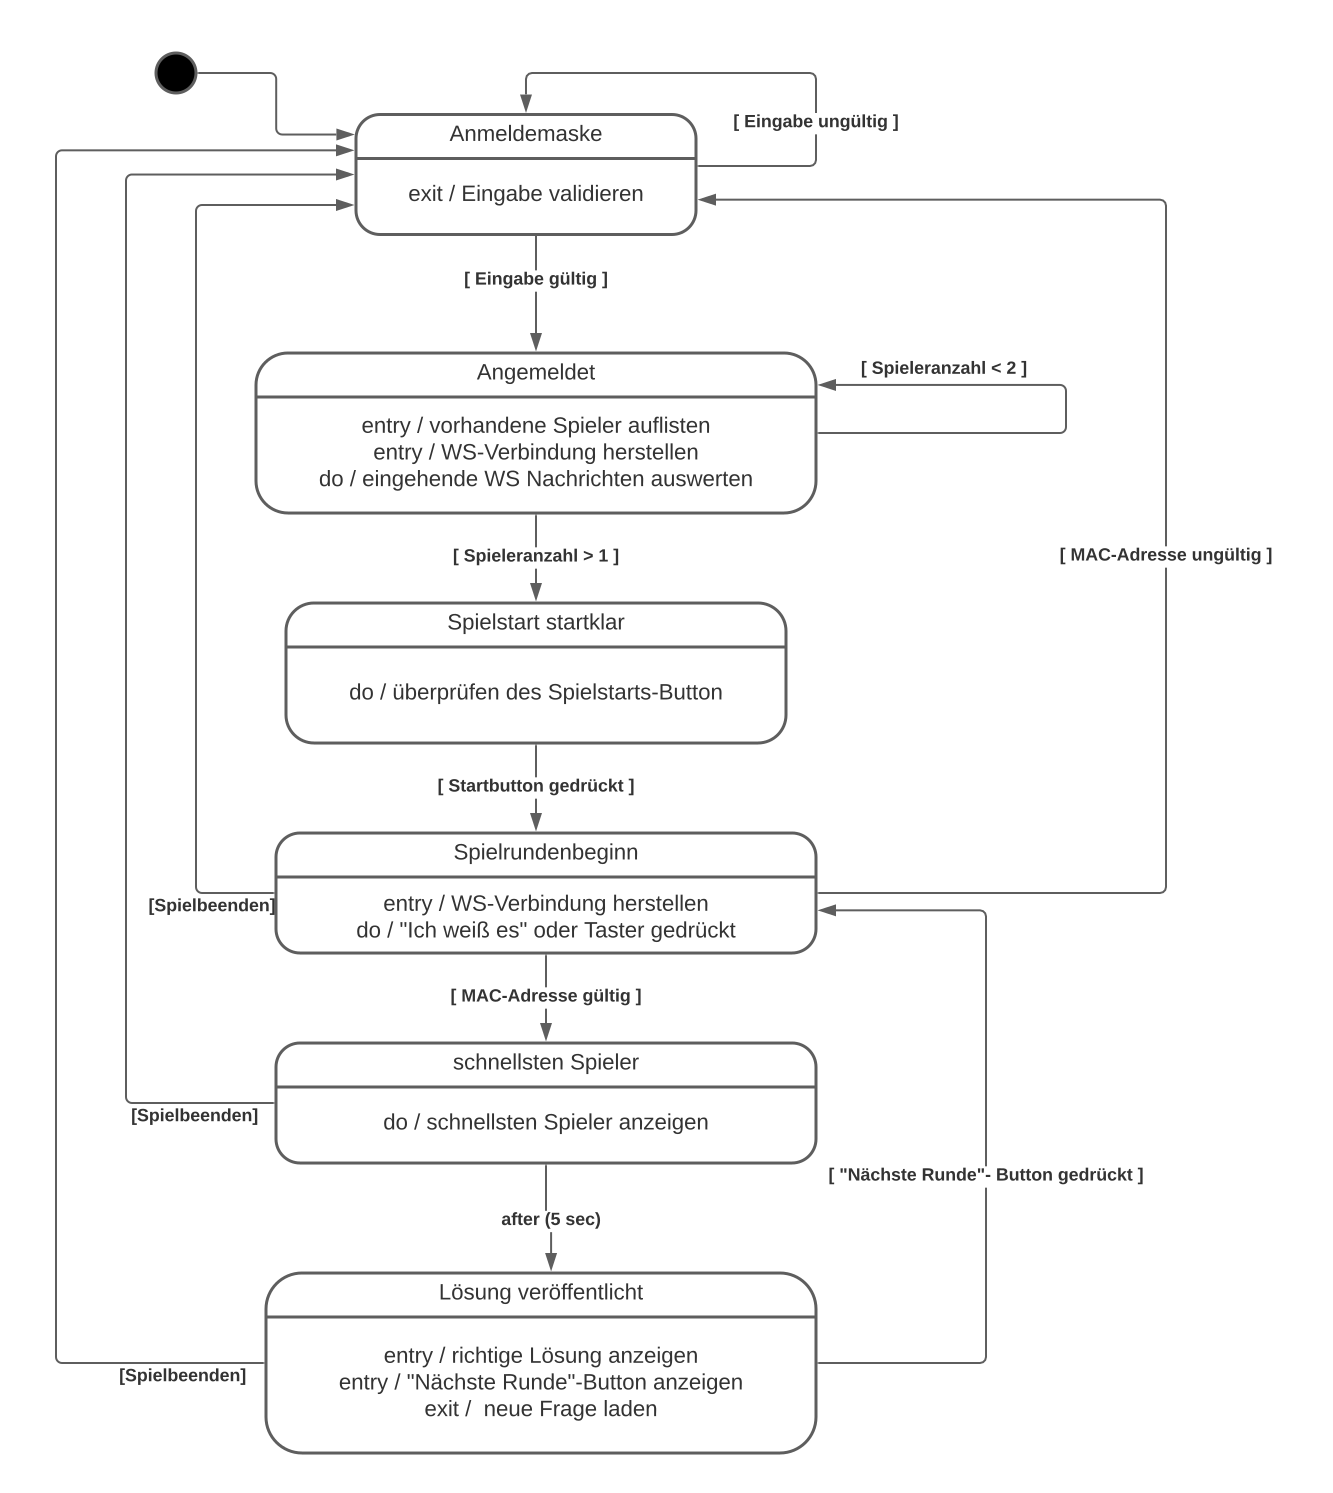
\includegraphics[width=24cm]{abbildungen/Zustandsdiagramm.png}    
    \captionof{figure}{Zustandsdiagramm}
  \end{center}
  \subsection*{Analyse und kritische Betrachtung der Ergebnisse}
  \Large\input{fazit.txt}
%  \renewcommand\refname{Referenzen}
%  \footnotesize\bibliography{literatur.bib}

\end{multicols*}
\end{document}
